\documentclass{beamer}
\mode<presentation>{
  \usetheme{Boadilla}
  \usefonttheme[onlylarge]{structurebold}
  \usefonttheme[stillsansseriflarge]{serif}
  \setbeamerfont*{frametitle}{size=\normalsize,series=\bfseries}
  % \setbeamertemplate{navigation symbols}{}
  \setbeamercovered{transparent}
}
\usepackage[english]{babel}
\usepackage[latin1]{inputenc}
\usepackage{times}
\usepackage[T1]{fontenc}
\usepackage{amsmath}
\usepackage{amssymb}
\usepackage{esint}
\usepackage{hyperref}
\usepackage{tikz}
\usepackage{xkeyval}
\usepackage{xargs}
\usepackage{verbatim}
\usetikzlibrary{
  arrows,
  calc,
  decorations.pathmorphing,
  decorations.pathreplacing,
  decorations.markings,
  fadings,
  positioning,
  shapes
}

\mode<handout>{
  \usepackage{pgfpages}
  \pgfpagesuselayout{4 on 1}[a4paper,landscape,border shrink=5mm]
  \setbeamercolor{background canvas}{bg=black!10}
}

\newcommand\pgfmathsinandcos[3]{%
  \pgfmathsetmacro#1{sin(#3)}%
  \pgfmathsetmacro#2{cos(#3)}%
}
\newcommand\LongitudePlane[3][current plane]{%
  \pgfmathsinandcos\sinEl\cosEl{#2} % elevation
  \pgfmathsinandcos\sint\cost{#3} % azimuth
  \tikzset{#1/.estyle={cm={\cost,\sint*\sinEl,0,\cosEl,(0,0)}}}
}
\newcommand\LatitudePlane[3][current plane]{%
  \pgfmathsinandcos\sinEl\cosEl{#2} % elevation
  \pgfmathsinandcos\sint\cost{#3} % latitude
  \pgfmathsetmacro\yshift{\cosEl*\sint}
  \tikzset{#1/.estyle={cm={\cost,0,0,\cost*\sinEl,(0,\yshift)}}} %
}
\newcommand\DrawLongitudeCircle[2][1]{
  \LongitudePlane{\angEl}{#2}
  \tikzset{current plane/.prefix style={scale=#1}}
  % angle of "visibility"
  \pgfmathsetmacro\angVis{atan(sin(#2)*cos(\angEl)/sin(\angEl))} %
  \draw[current plane] (\angVis:1) arc (\angVis:\angVis+180:1);
  \draw[current plane,dashed] (\angVis-180:1) arc (\angVis-180:\angVis:1);
}
\newcommand\DrawLatitudeCircleArrow[2][1]{
  \LatitudePlane{\angEl}{#2}
  \tikzset{current plane/.prefix style={scale=#1}}
  \pgfmathsetmacro\sinVis{sin(#2)/cos(#2)*sin(\angEl)/cos(\angEl)}
  % angle of "visibility"
  \pgfmathsetmacro\angVis{asin(min(1,max(\sinVis,-1)))}
  \draw[current plane,decoration={markings, mark=at position 0.6 with {\arrow{<}}},postaction={decorate},line width=.6mm] (\angVis:1) arc (\angVis:-\angVis-180:1);
  \draw[current plane,dashed,line width=.6mm] (180-\angVis:1) arc (180-\angVis:\angVis:1);
}
\newcommand\DrawLatitudeCircle[2][1]{
  \LatitudePlane{\angEl}{#2}
  \tikzset{current plane/.prefix style={scale=#1}}
  \pgfmathsetmacro\sinVis{sin(#2)/cos(#2)*sin(\angEl)/cos(\angEl)}
  % angle of "visibility"
  \pgfmathsetmacro\angVis{asin(min(1,max(\sinVis,-1)))}
  \draw[current plane] (\angVis:1) arc (\angVis:-\angVis-180:1);
  \draw[current plane,dashed] (180-\angVis:1) arc (180-\angVis:\angVis:1);
}
\newcommand\coil[1]{
  {\rh * cos(\t * pi r)}, {\apart * (2 * #1 + \t) + \rv * sin(\t * pi r)}
}
\makeatletter
\define@key{DrawFromCenter}{style}[{->}]{
  \tikzset{DrawFromCenterPlane/.style={#1}}
}
\define@key{DrawFromCenter}{r}[1]{
  \def\@R{#1}
}
\define@key{DrawFromCenter}{center}[(0, 0)]{
  \def\@Center{#1}
}
\define@key{DrawFromCenter}{theta}[0]{
  \def\@Theta{#1}
}
\define@key{DrawFromCenter}{phi}[0]{
  \def\@Phi{#1}
}
\presetkeys{DrawFromCenter}{style, r, center, theta, phi}{}
\newcommand*\DrawFromCenter[1][]{
  \setkeys{DrawFromCenter}{#1}{
    \pgfmathsinandcos\sint\cost{\@Theta}
    \pgfmathsinandcos\sinp\cosp{\@Phi}
    \pgfmathsinandcos\sinA\cosA{\angEl}
    \pgfmathsetmacro\DX{\@R*\cost*\cosp}
    \pgfmathsetmacro\DY{\@R*(\cost*\sinp*\sinA+\sint*\cosA)}
    \draw[DrawFromCenterPlane] \@Center -- ++(\DX, \DY);
  }
}
\newcommand*\DrawFromCenterText[2][]{
  \setkeys{DrawFromCenter}{#1}{
    \pgfmathsinandcos\sint\cost{\@Theta}
    \pgfmathsinandcos\sinp\cosp{\@Phi}
    \pgfmathsinandcos\sinA\cosA{\angEl}
    \pgfmathsetmacro\DX{\@R*\cost*\cosp}
    \pgfmathsetmacro\DY{\@R*(\cost*\sinp*\sinA+\sint*\cosA)}
    \draw[DrawFromCenterPlane] \@Center -- ++(\DX, \DY) node {#2};
  }
}
\makeatother

% not mandatory, but I though it was better to set it blank
\setbeamertemplate{headline}{}
\def\beamer@entrycode{\vspace{-\headheight}}

\tikzstyle{snakearrow} = [decorate, decoration={pre length=0.2cm,
  post length=0.2cm, snake, amplitude=.4mm,
  segment length=2mm},thick, ->]

%% document-wide tikz options and styles

\tikzset{%
  >=latex, % option for nice arrows
  inner sep=0pt,%
  outer sep=2pt,%
  mark coordinate/.style={inner sep=0pt,outer sep=0pt,minimum size=3pt,
    fill=black,circle}%
}
\def\timeleft{15:00->14:55}

\title[Doppler-free spectroscopy using saturated absorption\hspace{2em}\tiny{\timeleft}]{Doppler-free spectroscopy}
\author{Yichao Yu}
\institute{MIT}

\begin{document}

\begin{frame}{}
  \titlepage
\end{frame}

% Intro
\def\timeleft{14:55->14:20}
\begin{frame}{Introduction}
  \begin{block}{}
    \begin{itemize}[<+->]
    \item
      Saturated absorption.
    \item
      Precise spectrum measurement.
    \item
      Frequency stabilization and locking.
    \end{itemize}
  \end{block}
\end{frame}

\def\timeleft{14:20->13:50}
\begin{frame}
  \tableofcontents
\end{frame}

\def\timeleft{13:50->11:40}
% Theory
\section{Saturated absorption and atom hyperfine structure.}
\begin{frame}{Doppler broadening and spectral hole buning.}
  \begin{columns}
    \column{6cm}
    \begin{block}{}
      \begin{itemize}[<+->]
      \item
        Natural line width.
      \item
        Doppler broadening.
        \[ \Delta f=\frac{v}{c}f_0\approx100MHz \]
      \item
        Cooling.
      \item
        Saturated absorption: whole burning without doppler broadening.
      \end{itemize}
    \end{block}
    \column{6cm}
    \begin{tikzpicture}[scale=.8]
      \draw[smooth,domain=-2.5:2.5] plot function{2*exp(-x**2)};
      \draw[smooth,domain=-2.5:2.5,dashed] plot function{2*exp(-x**2)};
      \draw[smooth,domain=-2.5:2.5] plot function{2*exp(-x**2)-1.2*exp(-x**2 * 40)};
      \draw[->,black] (-3,0) -- (3,0) node[right] {$f$};
      \draw[->,black] (0,0) -- (0,3);
    \end{tikzpicture}
  \end{columns}
\end{frame}

\def\timeleft{10:00 -> 7:30}
% apparatus
\section{Apparatus and measurement.}
\begin{frame}{Apparatus.}
  \begin{center}
    \begin{tikzpicture}[scale=.8]
      \draw[line width=.2, dashed, red] (0, 0) -- (3, 1) -- (7, 1) -- (9, 0);
      \draw[line width=.2, dashed, red] (0, 0) -- (3, -1) -- (7, -1) -- (9, 0);
      \draw[line width=.2, dashed, red] (0, 0) -- (3, 0) -- (7, 0) -- (9, 0);

      \draw (0, 0) circle (.2);
      \path (0, -.3) node[below] {$Rb$ Lamp};

      \draw[line width=1.2] (1, -1) -- (1, 1) node[above] {{\visible<2->{$P$}}};
      \draw[line width=1.2] (2, -1) -- (2, 1) node[above] {{\visible<2->{$\dfrac{\lambda}{4}$}}};
      \draw[line width=1.2, <->] (3, -1) -- (3, 1);

      \draw (5, 0) circle (.6) node {{\visible<3->{$Rb$}}};

      \visible<5->{
        \draw (5, .7) ellipse (.7 and .05);
        \draw (5, -.7) ellipse (.7 and .05);
        \path (5, -.75) node[below] {rf};
      }

      \visible<4->{
        \draw[line width=2, brown] (4, 0) ellipse (.3 and 1.7);
        \draw[line width=2, brown] (6, 0) ellipse (.3 and 1.7);
        \path (5, 1.7) node[above] {$B$};
      }

      \draw[line width=1.2, <->] (7, -1) -- (7, 1);
      \draw (9, 0) circle (.2);
      \path (9, -.3) node[below] {Detector};
    \end{tikzpicture}
  \end{center}
  \begin{block}{}
    \begin{itemize}
    \item<2->
      Circular polarization.
    \item<3->
      ${}^{85}Rb$ and ${}^{87}Rb$
    \item<4->
      $B$ field.
    \item<5->
      RF field.
    \end{itemize}
  \end{block}
\end{frame}

\def\timeleft{7:30 -> 4:00}
% goal
\begin{frame}{Measurement}
  \visible<+->{
    \begin{block}{}
      \[ \Delta\mu B=hf \]
      \uncover<+->{
        \[ f_{RF}=\frac{g_F\mu_B}{h}\sqrt{(B_x+B_{x0})^2+(B_y+B_{y0})^2+(B_z+B_{z0})^2} \]
      }
    \end{block}
  }
  \begin{columns}
    \column{5.5cm}
    \begin{block}{}
      \begin{itemize}[<+->]
      \item
        Scan RF frequency.
      \item
        Scan $B$ field.
      \item
        Switch $B$ field.
      \end{itemize}
    \end{block}
    \column{5.5cm}
    \only<3>{
      \begin{block}{Scaning RF frequency at different $B$ field.}
        \begin{itemize}
        \item
          Measure/cancel earth magnetic field.
        \item
          Natural Abundance. \alert{Different from the strength of the absorption.}
          \[ I_{absorb}\propto NA\cdot g_F^2 \]
        \end{itemize}
      \end{block}
    }
    \only<4>{
      \begin{block}{Scan $B$ field at different RF frequency.}
        \begin{itemize}
        \item
          Measure resonance frequency.
        \end{itemize}
      \end{block}
    }
    \only<5>{
      \begin{block}{Switch $B$ at different light intensity.}
        \begin{itemize}
        \item
          Measure pumping rate.
          \[ R\propto I_{light} \]
        \end{itemize}
      \end{block}
    }
  \end{columns}
\end{frame}

\def\timeleft{4:00->3:00}
\section{Data and result.}
\begin{frame}{Scanning $B$ field.}
  \begin{columns}
    \column{6cm}
    % 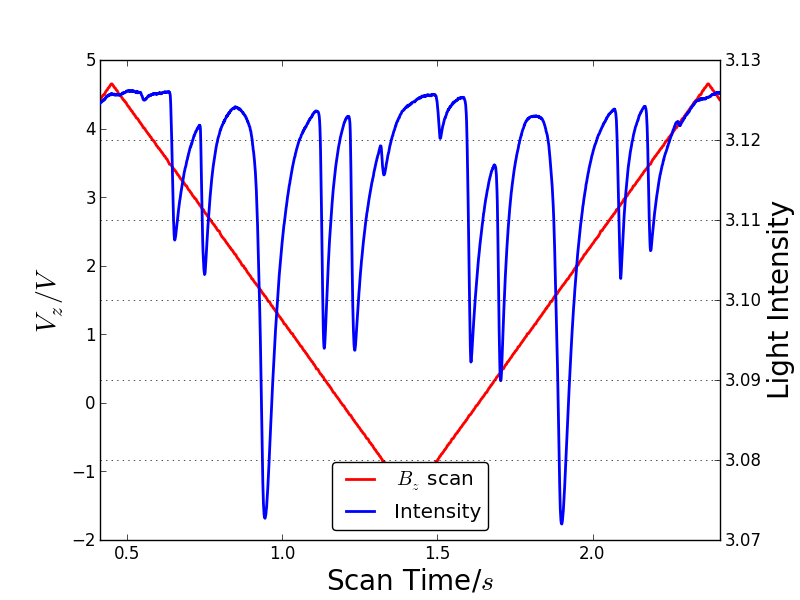
\includegraphics[width=6cm]{../bscan_nf/03-15-bscan_nf_rf1.png}\\
    Light intensity when scanning $B$ field.
    \column{6cm}
    \only<2>{
      \begin{block}{$g_F$ factor.}
        \begin{center}
          \begin{tabular}{|c|c|c|}
            \hline
            Isotrope&Measured&Expected\\\hline
            ${}^{85}Rb$&$0.498(19)$&$0.500$\\\hline
            ${}^{87}Rb$&$0.331(13)$&$0.333$\\\hline
          \end{tabular}
        \end{center}
      \end{block}
    }
  \end{columns}
\end{frame}

\begin{frame}{Scanning RF frequency.}
  \begin{columns}
    \column{6cm}
    % 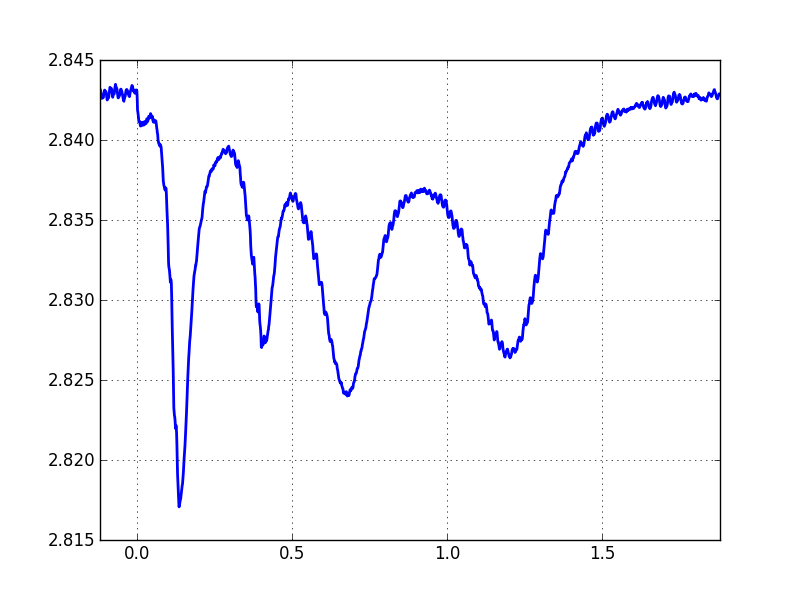
\includegraphics[width=6cm]{../rfscan_nf/03-19-rfscan_nf_y7.png}\\
    Light intensity when scanning RF frequency.
    \column{6cm}
    \only<2>{
      % 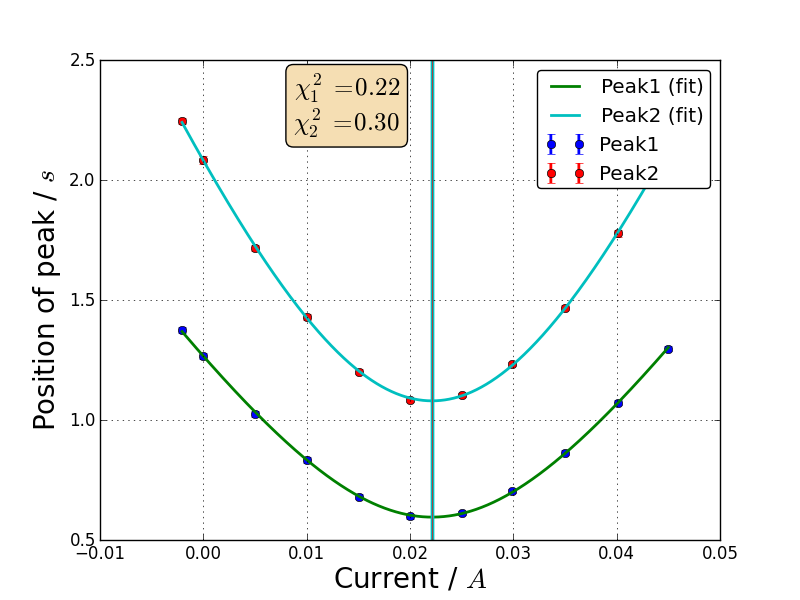
\includegraphics[width=6cm]{../rfscan_nf/rfscan_y_fit.png}\\
      Peak positions at different $y$ current
      \begin{block}{Ambient magnetic field.}
        \begin{center}
          \begin{tabular}{|c|c|}
            \hline
            $B_x/mGs$&$361(10)$\\\hline
            $B_y/mGs$&$72.2(1.6)$\\\hline
            $B_z/mGs$&$191.6(5.2)$\\\hline
          \end{tabular}
        \end{center}
      \end{block}
    }
    \only<3>{
      \begin{block}{Natural Abundance.}
        \begin{center}
          \begin{tabular}{|c|c|c|}
            \hline
            Isotrope&Measured&Expected\\\hline
            ${}^{85}Rb$&$72.0(2.2)\%$&$72.168\%$\\\hline
            ${}^{87}Rb$&$28.0(2.2)\%$&$27.835\%$\\\hline
          \end{tabular}
        \end{center}
      \end{block}
    }
  \end{columns}
\end{frame}

\def\timeleft{0:30->0:00}
\section{Conclusion.}
\begin{frame}{Conclusion.}
  \begin{block}{}
    \begin{itemize}[<+->]
    \item
      Observed optical pumping and depolarization.
    \item
      Ambient megnetic field.
    \item
      $g_F$ factors.
    \item
      Natural abundance of ${}^{85}Rb$ and  ${}^{87}Rb$.
    \end{itemize}
  \end{block}
\end{frame}

\begin{frame}{}
\end{frame}

\begin{frame}{}
  \begin{block}{Land� g-factor}
    \[g_J\approx\frac{3}{2}+\frac{S(S+1)-L(L+1)}{2J(J+1)}\]
    \[g_F\approx g_J\frac{F(F+1)-I(I+1)+J(J+1)}{2F(F+1)}\]
  \end{block}
  \begin{columns}
    \column{5.5cm}
    \begin{block}{}
      \begin{center}
        $S=\dfrac12$\qquad$L=0$\qquad$J=\frac12$\\
        $I=\left\{\begin{array}{ll}
            \dfrac52&({}^{85}Rb)\\
            \dfrac32&({}^{87}Rb)
          \end{array}
        \right.$
        $F=\left\{\begin{array}{ll}
            3&({}^{85}Rb)\\
            2&({}^{87}Rb)
          \end{array}
        \right.$
      \end{center}
    \end{block}
    \column{5.5cm}
    \begin{block}{}
      \begin{center}
        $g_F=\left\{\begin{array}{ll}
            \dfrac13&(Rb^{85})\\
            \dfrac12&(Rb^{87})
          \end{array}
        \right.$
      \end{center}
    \end{block}
  \end{columns}
\end{frame}

\end{document}
